
\documentclass{beamer}
\usetheme{CambridgeUS}
\setbeamertemplate{blocks}[rounded][shadow=true]

% Color settings
\setbeamercolor{title}{bg=red!65!black, fg=white}

\setbeamercolor{block title}{use=structure,fg=white,bg=red!65!black}
\setbeamercolor{block body}{use=structure,fg=black,bg=black!3}

\setbeamercolor*{block title example}{fg=blue!50!black,bg=blue!10!white}
\setbeamercolor*{block body example}{fg=black,bg=blue!2}

% Margin
\setbeamersize{text margin left=30pt,text margin right=30pt}

\graphicspath{ {bilder/} }

% \AtBeginSection[]{%
% 	\begin{frame}
% 		\tableofcontents[currentsection]
% 	\end{frame}
% }% AtBeginSection



\mode<presentation>
{
\setbeamercovered{transparent}
}
\usepackage{amsmath,amsfonts,amssymb}
\usepackage[center]{caption}
\usepackage[utf8]{inputenc}
\usepackage[ngerman]{babel}
\usepackage{graphicx}
\usepackage{svg}
\usepackage{pdfpages}
\usepackage{placeins}
\usepackage[decimalsymbol=comma]{siunitx}

\usepackage{svg}
\usepackage{changepage}

\usepackage{mathptmx}
\usepackage[scaled=.90]{helvet}
\usepackage{courier}
\beamertemplatenavigationsymbolsempty 
\setbeamertemplate{footline}{}

%\usepackage[T1]{fontenc}
\title{Spurdetektoren}
\author[V. Grimm]{Verena Grimm}


\institute[]{
Seminarvortrag\\
Fachbereich Physik, Mathematik und Informatik (FB 08)\\
Johannes Gutenberg-Universität Mainz
}

\date{04.11.2014}


% Logo Universität
\titlegraphic{
\includegraphics[width=4cm]{bilder/JGU-Logo_sw_high.jpg}\hspace*{-8.5cm}}




\begin{document}

\begin{frame}
\titlepage
\end{frame}

\begin{frame}
\frametitle{Inhalt}
\tableofcontents
\end{frame}

\subsection[]{Driftkammer}

\begin{frame}{Driftkammer}
    \begin{columns}[T]
	    \column{.5\textwidth}
			\begin{figure}[htbp]
			  \centering
			  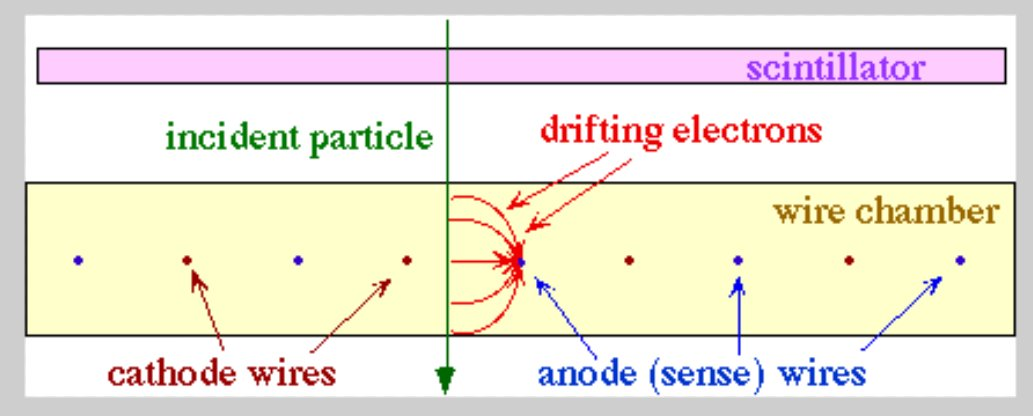
\includegraphics[width=\textwidth]{drift.jpg}
			  \caption{Aufbau einer Driftkammer}
			\end{figure}
			
	    \column{.55\textwidth}
	    	\begin{itemize}
	    	  \item Messung der Ortsinformation durch Messung der Driftzeit
			  \item Aufbau: Proportionalzähler mit Trigger (Szintillator $\rightarrow$ schnelles Signal)
			  \item Trigger gibt den Zeitpunkt $t_0$, an dem Teilchen eintrifft
			  \item Anode gibt den Zeitpunkt $t_1$, an dem Signal (Elektronen) eintrifft
			  \item bei bekannter Driftgeschw. $u$: Distanz von Enstehungsort zu Anode ist
			  $x=\int_{t_0}^{t_1}u\cdot dt$
			\end{itemize}
			
    \end{columns}
\end{frame}

\begin{frame}{Driftkammer}

	\begin{block}{Wie kommt die Spur zustande?}
		\begin{itemize}
		  \item mehrere Ebenen hintereinander, um Spur zu rekonstruieren
		  \item verschiedene Orientierungen der Drähte
		\end{itemize}
	\end{block}
	\vspace{0.8cm}
    \begin{columns}[T]
		\column{.45\textwidth}
			Vorteile		
			\begin{itemize}
			  \item großflächiger Aufbau möglich
			  \item wenige Kanäle
			  \item gute Ortsauflösung ($O(100\mu m)$)
			\end{itemize}	
	    \column{.5\textwidth}
	    	Nachteile
	    	\begin{itemize}
			  \item Größerer Abstand der Drähte $\rightarrow$ höhere Rate pro Draht 
			\end{itemize}
    \end{columns}
    \vspace{1cm}
\end{frame}

\begin{frame}{Driftkammer}
    Beispielbild?
\end{frame}



%___________________________________________________________________________________________________
%___________________________________________________________________________________________________
%___________________________________________________________________________________________________

\section{Halbleiterdetektoren}
\subsection[]{Grundlagen}

\begin{frame}{Grundlagen}
    \begin{columns}[T]
	    \column{.57\textwidth}
	    	\vspace{-0.5cm}
			\begin{figure}[htbp]
			  \centering
			  \includesvg[svgpath=bilder/, width=\columnwidth]{diode-pnuebergang}
			\end{figure}
			\vspace{-1.2cm}
			\begin{figure}[htbp]
			  \centering
			   \includesvg[svgpath=bilder/, width=\columnwidth]{diode-sperrschicht}
			   \vspace{-0.5cm}
			  \caption{pn-Übergang einer Diode}
			\end{figure}
			
	    \column{.4\textwidth}
	    	\begin{itemize}
	    	  \item Diode: Übergang zwischen n-dotierter zu p-dotierter Schicht
			  \item Ausbilden einer Raumladungszone durch Diffusion der freien Ladungsträger
			  \item Spannung in Sperrrichtung: kein Stromfluss möglich
			\end{itemize}
    \end{columns}
\end{frame}

\begin{frame}{Grundlagen}
    \begin{columns}[T]	
	    \column{.45\textwidth}
	    	\begin{itemize}
	    	  \item eintreffende Strahlung erzeugt $e^-$/Loch-Paare: $e^-$ werden ins Leitungsband
	    	  gehoben, Löcher bleiben im Valenzband zurück
	    	  \item ca. 3~eV nötig, um ein $e^-$/Loch-Paar zu erzeugen
	    	  \item Diffusion der freien $e^-$ zur Anode, Diffusion der Löcher zur Kathode $\rightarrow$
	    	  messbarer Strom $\propto$ Energie des Teilchens
			\end{itemize}
			
		\column{.5\textwidth}
			\begin{figure}[htbp]
			  \centering
			   \includesvg[svgpath=bilder/, width=\columnwidth]{diode-detektor}
			  \caption{pn-Übergang einer Diode}
			\end{figure}
    \end{columns}
\end{frame}
\subsection[]{Pixel- und Streifendetektoren}


\begin{frame}{Streifendetektoren}
	\begin{columns}[T]
		\column{.45\textwidth}
			\begin{figure}[htbp]
			  \centering
			   \includesvg[svgpath=bilder/, width=\textwidth]{streifen}
			  \caption{Schema Streifendetektor}
			\end{figure}
	    \column{.5\textwidth}
	    	\begin{itemize}
			  \item Meist n-dotiertes Grundmaterial mit p-dotierten Streifen
			  \item Streifenbreite 10-100 $\mu$m
			  \item einseitiger Streifendetektor $\rightarrow$ eindim. Ortsinformation
			  \item doppelseitig: Elektroden in nicht-parallele Streifen segmentieren (meist 90$^\circ$)
			  $\rightarrow$ zweidim. Ortsinformation
			\end{itemize}
    \end{columns}
\end{frame}

\begin{frame}{Pixeldetektoren}
	\begin{columns}[T]
		\column{.45\textwidth}
			\begin{figure}[htbp]
			  \centering
			  \includesvg[svgpath=bilder/, width=\textwidth]{pixel}
			  \caption{Schema Pixeldetektor}
			\end{figure}	
	    \column{.5\textwidth}
	    	\begin{itemize}
			  \item Elektroden in rechteckige Pixel segmentiert $\rightarrow$ zweidim. Ortsinformation
			  \item kleinere Elektrodenoberfläche besser um Signal zu verarbeiten (kleinerer Leckstrom)
			  \item hohe Kanalzahl
			\end{itemize}
    \end{columns}
\end{frame}


\begin{frame}{Pixeldetektoren}
			\begin{figure}[htbp]
			  \centering
			  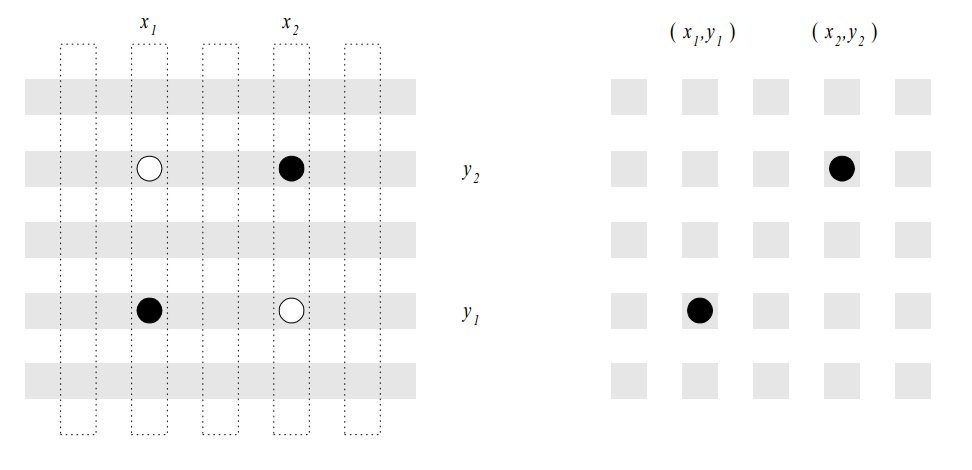
\includegraphics[width=\textwidth]{pixelstreifenvgl.jpg}
			  \caption{Mehrfachtreffer in doppelseitigem Streifendetektor erzeugen Mehrdeutigkeiten bei Zuordnung
			Trefferkoordinaten [gsp]}
			\end{figure}	
% 			 \vspace{1cm}			
\end{frame}


\begin{frame}{Pixel-/Streifendetektoren}
    \begin{columns}[T]
		\column{.45\textwidth}
			\textbf{Vorteile}		
			\begin{itemize}
			  \item gute Ortsauflösung $O(10\mu m)$  ($<$~MWPC/Driftkammer, aber Pixel~$<$~Streifen)
			  \item kleinere Energie, um $e^-$/Loch-Paar zu erzeugen $\rightarrow$ kleinere Variation der
			  Pulshöhe, höhere Energieauflösung
			  \item Pixeldetektoren erlauben eindeutige Zuordnung
			\end{itemize}	
	    \column{.5\textwidth}
	    	\textbf{Nachteile}
	    	\begin{itemize}
			  \item teuer
			  \item hohe Verlustleistung (Kühlung notwendig)
			  \item begrenzte Haltbarkeit bei hoher Strahlung (nicht ionisierende Strahlung $\rightarrow$
			  z.B. Leerstellen im Gitter)
			\end{itemize}
    \end{columns}
   \end{frame}
   
%    \begin{frame}{Pixeldetektoren}
% 			\begin{figure}[htbp]
% 			  \centering
% 			  \includegraphics[width=\textwidth*0.5]{bla.jpg}
% 			  \caption{beispielbild}
% 			\end{figure}	
% % 			 \vspace{1cm}			
% \end{frame}

%___________________________________________________________________________________________________
%___________________________________________________________________________________________________
%___________________________________________________________________________________________________

\section{Szintillationsdetektoren}
\subsection[]{Grundlagen}

\begin{frame}{Szintillatoren}

\begin{description}
	  \item[Szintillatoren] bestehen aus Material, dessen Moleküle nach Anregung durch geladene
	  Teilchen oder Photonen die Anregungsenergie in Form von Licht wieder abgeben
	\end{description}
	\begin{block}{Arten}
		\begin{itemize}
		  \item organische Szintillatoren (Kristalle, Gläser, Edelgase)
		  \item anorganische Szintillatoren (Kristalle, Flüssigkeiten, Plastik)
		\end{itemize}
	\end{block}
	\vspace{0.7cm}
	Auslese i.d.R. durch Photomultiplier
\end{frame}	


\begin{frame}{Szintillatoren}
	\begin{block}{Anorganische Szintillatoren}
		\begin{itemize}
		  \item anorganische Kristalle mit eingebrachten Fremdatomen (Aktivatorzentren) $\rightarrow$
		  zusätzliche Energieniveaus
		  \item durch eintreffende Strahlung angeregtes $e^-$ wandert durch Kristall, bis es auf Loch
		  trifft und rekombiniert $\rightarrow$ Abgabe eines Photons
		  \item Bsp.: NaI,CsI, BaF$_2$,
		\end{itemize}
	\end{block}
		\begin{block}{Organische Szintillatoren}
		\begin{itemize}
		  \item aromatische Kohlenwasserstoffverbindungen
		  \item hauptsächlich organische Kristalle oder Plastikszintillatoren
		  \item Wechsel eines freien Valenzelektrons zw.
Molekülorbitalen verschiedener Energie unter Abgabe eines Photons
		  \item Bsp.: C$_{10}$H$_8$, C$_{14}$H$_{10}$
		\end{itemize}
	\end{block}
\end{frame}	

	
\subsection[]{Szintillationszähler}



\begin{frame}{Szintillationszähler}
	\begin{columns}[T]
		\column{.65\textwidth}
			\begin{itemize}
			  \item Bündelung von Szintillationsfasern ($\varnothing~<$~1~mm)
			  \item parallele Bündel ergeben eindimensionale Ortsinformation
			  \item senkrecht aufeinander stehende Ebenen ergeben zwei- bzw. dreidimensionale Ortsinformation
			  \item oft 1-2 Mäntel um Fasern, um Lichtausbeute zu erhöhen
			  \item Anordnung der Faser je nach Detektorgeometrie
			\end{itemize}	
	    \column{.4\textwidth}
	    	\begin{figure}[htbp]
			  \centering
			  \includesvg[svgpath=bilder/, width=\columnwidth]{szintillator-fasern}
% 			  \caption{Aufbau eines Szintillationszählers}
			\end{figure}
    \end{columns}
\end{frame}	
	
	\begin{frame}{Szintillationszähler}
    \begin{columns}[T]
		\column{.45\textwidth}
			\textbf{Vorteile}		
			\vspace{0.7cm}
			\begin{itemize}
			  \item 
			\end{itemize}	
	    \column{.5\textwidth}
	    	\textbf{Nachteile}
	    	\vspace{0.7cm}
	    	\begin{itemize}
			  \item 
			\end{itemize}
    \end{columns}
\end{frame}

%___________________________________________________________________________________________________
%___________________________________________________________________________________________________
%___________________________________________________________________________________________________
\AtBeginSection[]{%
	\begin{frame}
		\tableofcontents[currentsection]
	\end{frame}
}% AtBeginSection
\section{Zusammenfassung und Vergleich}


\begin{frame}{Zusammenfassung und Vergleich}
	
	\begin{block}{Gasdetektoren}
	\end{block}
	
	\begin{block}{Halbleiterdetektoren}
	
	\end{block}

\end{frame}


\begin{frame}{Was gibt es noch?}
	
	\begin{block}{Detektoren}
		\begin{itemize}
		  \item Liquid Ionisation Detectors (z.B. Blasenkammer)
		  \item TPC (Time Projection Chamber)
		  \item GEMs (Gas Electron Multiplier), MicroMegas (Micro-Mesh Gaseous Structure)
		  \item Szintillatioren (Hodoskope)
		  \item \ldots
		\end{itemize}
	\end{block}
	
		\begin{block}{Spurrekonstruktion}
		\begin{itemize}
		  \item Hough-Transformation
		  \item Kalman-Filter
		\end{itemize}
	\end{block}

\end{frame}
%___________________________________________________________________________________________________
%___________________________________________________________________________________________________
% \section{Spurrekonstruktion}
% \subsection{Hough-Transformation}


%___________________________________________________________________________________________________

\begin{frame}{Abbildungsverzeichnis}
\footnotesize
	\begin{adjustwidth}{-5em}{-2em}
	  	\begin{description}
		  	\item[wbk]
		  	https://de.wikipedia.org/w/index.php?title=Datei:Blasenkammer.svg
		  	\item[gfa]
		  	http://www.rapp-instruments.de/Radioaktivitaet/Funkenkammer/multigap/spark.htm
		  	\item[gfk]
		  	http://kworkquark.desy.de/lexikon/lexikon.funkenkammer/0/
		  	\item[gnk]
		  	http://www2.slgb.ch/users/soe/Physik/Hochenergie/teilchen/teilchen.htm
		  	\item[wzr]
		  	https://de.wikipedia.org/wiki/Datei:Geiger\_Mueller\_Counter\_with\_Circuit-de.svg
		  	\item[wzk]
			http://de.wikipedia.org/wiki/Datei:Kennlinie\_Zaehlrohr-GER.svg
			\item[wvk]
		  	http://de.wikipedia.org/wiki/Drahtkammer\#mediaviewer/File:Wire\_ chamber\_schematic.svg
		  	\item[wvkf]
		  	http://upload.wikimedia.org/wikipedia/commons/2/22/Wire\_chamber\_E\_field.svg
		  	\item[cpu]
		  	http://francis.naukas.com/2012/06/16/ya-hay-colisiones-proton-proton-en-el-lhc-que-presentan-mas-de-30-vertices-apilados/
		  	\item[gpn]
		  	http://elektronik-kurs.net/wp-content/uploads/2012/05/Bildschirmfoto-2012-05-30-um-14.28.03.png
		  	\item[gsp]
		  	https://mkeil.web.cern.ch/mkeil/papers/diss.pdf
		\end{description}
	\end{adjustwidth}  
\end{frame}

\end{document}